



%----------------------------------------------------------------------------------------

\newpage



\section{Real Estate Transactions}{Transactions immobilières et Grand Paris}

\label{sec:grandparisrealestate}


%----------------------------------------------------------------------------------------



%%%%%%%%%%%%%
\subsection{Context}{Contexte}



\bpar{
Various aspects of territories are concerned by interactions with networks. In previous empirical studies, no socio-economic attributes of populations inhabiting the territory nor economic values for land and real estate was considered. Both are however crucial elements of territorial dynamics and are extensively studied in fields such as territorial analysis or urban economics : for example, \cite{homocianu:tel-00359302} studies households residential choices to understand land-use transportation interactions. We propose here to use a database of Real Estate transactions for Parisian region on the last 20 years, with 2 years temporal granularity and exact spatial coordinates. \cite{guerois2009dynamique} used it to make typologies of spatial dynamics of Parisian real estate.
}{
Des aspects très variés des territoires sont concernés par l'interaction avec les réseaux. Dans nos études précédentes, les aspects économiques et financiers du foncier et l'immobilier n'ont pas été considérés. Il s'agit cependant d'éléments cruciaux des dynamiques territoriales et sont étudiés de manière intensive dans des champs comme l'analyse territoriale ou l'économie urbaine : par exemple, \cite{homocianu:tel-00359302} étudie les choix résidentiels des ménages pour comprendre les interactions entre usage du sol et transport. Nous proposons ici d'utiliser entre autres une base de données de transactions immobilières pour la région parisienne sur les 20 dernières années, avec une granularité temporelle de 2 ans et coordonnées spatiales exactes. \cite{guerois2009dynamique} l'utilise par exemple pour établir une typologie des dynamiques spatiales du marché immobilier parisien.
}


Notre approche peut être comprise comme une recherche de signes précurseurs de rupture de potentiels du réseau: en effet, si des dynamiques territoriales intrinsèques anticipent l'arrivée d'une nouvelle station de transports en commun, les implications seront bien différentes du cas où celle-ci conduit ces variables après sa construction. L'interprétation en termes ``d'effets structurants'' sera notamment très différente. Nous appliquons ici la méthode de causalités spatio-temporelles

La région métropolitaine de Paris est en train de connaître de grandes mutations, avec la mise en place d'une gouvernance métropolitaine et de nouvelles infrastructures de transport par exemple. La construction d'un réseau de métro en rocade permettant des liaisons de banlieue à banlieue est un besoin ancien, et a mené à plusieurs propositions sur lesquelles se sont opposés l'Etat et la Région au tournant des années 2010~\cite{desjardins2010bataille}. Le projet Arc Express~\cite{stif2007arc}, porté par la Région et plus axé sur une égalité des territoires, contrastait avec les propositions initiales de Réseau du Grand Paris visant à relier des ``clusters d'excellence'' en dépit d'un possible effet tunnel. La solution finalement adoptée (voir le dernier schéma directeur \cite{sdrif2013}) est un compromis et permet un rééquilibrage est-ouest de l'accessibilité~\cite{beaucire2013grand}. Nous proposons d'étudier les relations entre différentiel d'accessibilité pour chaque projet, et variables liées au foncier (transactions immobilières) et socio-économiques. En effet, les liens entre nouvelles lignes et évolution du foncier sont parfois remarquables~\cite{damm1980response}.





%%%%%%%%%%%%%%%
\subsection{Case study}{Cas d'étude}





\subsubsection{Data}{Données}

Les données des transactions immobilières sont fournies par la base BIENS (Chambre des Notaires d'Ile de France, base propriétaire). Le nombre de transactions utilisables après nettoyage est de 862360, se répartissant sur l'ensemble des IRIS, pour une plage temporelle couvrant de 2003 à 2012 incluses. Les données par IRIS pour population et revenu (revenu médian et indice de Gini) proviennent de l'INSEE. Les données de réseau ont été vectorialisées à partir des cartes des projets (voir Fig.~\ref{fig:projects} pour les projets). Les temps de trajets sont calculés par transport en commun uniquement, avec des valeurs standard pour les vitesses moyennes des différents modes (RER 60km.h\textsuperscript{-1}, Transilien 100km.h\textsuperscript{-1}, Metro 30km.h\textsuperscript{-1}, Tramway 20km.h\textsuperscript{-1}). La matrice des temps est calculée depuis l'ensemble des centroïdes des IRIS vers l'ensemble des centroïdes des communes. Ceux-ci sont reliés au réseau par des connecteurs à la gare la plus proche, de vitesse 50km.h\textsuperscript{-1} (trajet en voiture). Les analyses sont implémentées intégralement en langage R~\cite{rcoreteam} et l'ensemble des données, du code source et des résulats sont disponibles sur un dépôt git ouvert\footnote{A l'adresse\\\texttt{https://github.com/JusteRaimbault/CityNetwork/tree/master/Models/SpatioTempCausality/GrandParis}. Les données de la base BIENS ne sont fournies que de manière agrégée à l'IRIS et pour les variables de prix et de crédit, pour des raisons de fermeture contractuelle de la base brute.}.




%%%%%%%%%%%%%%%
\begin{figure*}[h]
\centering
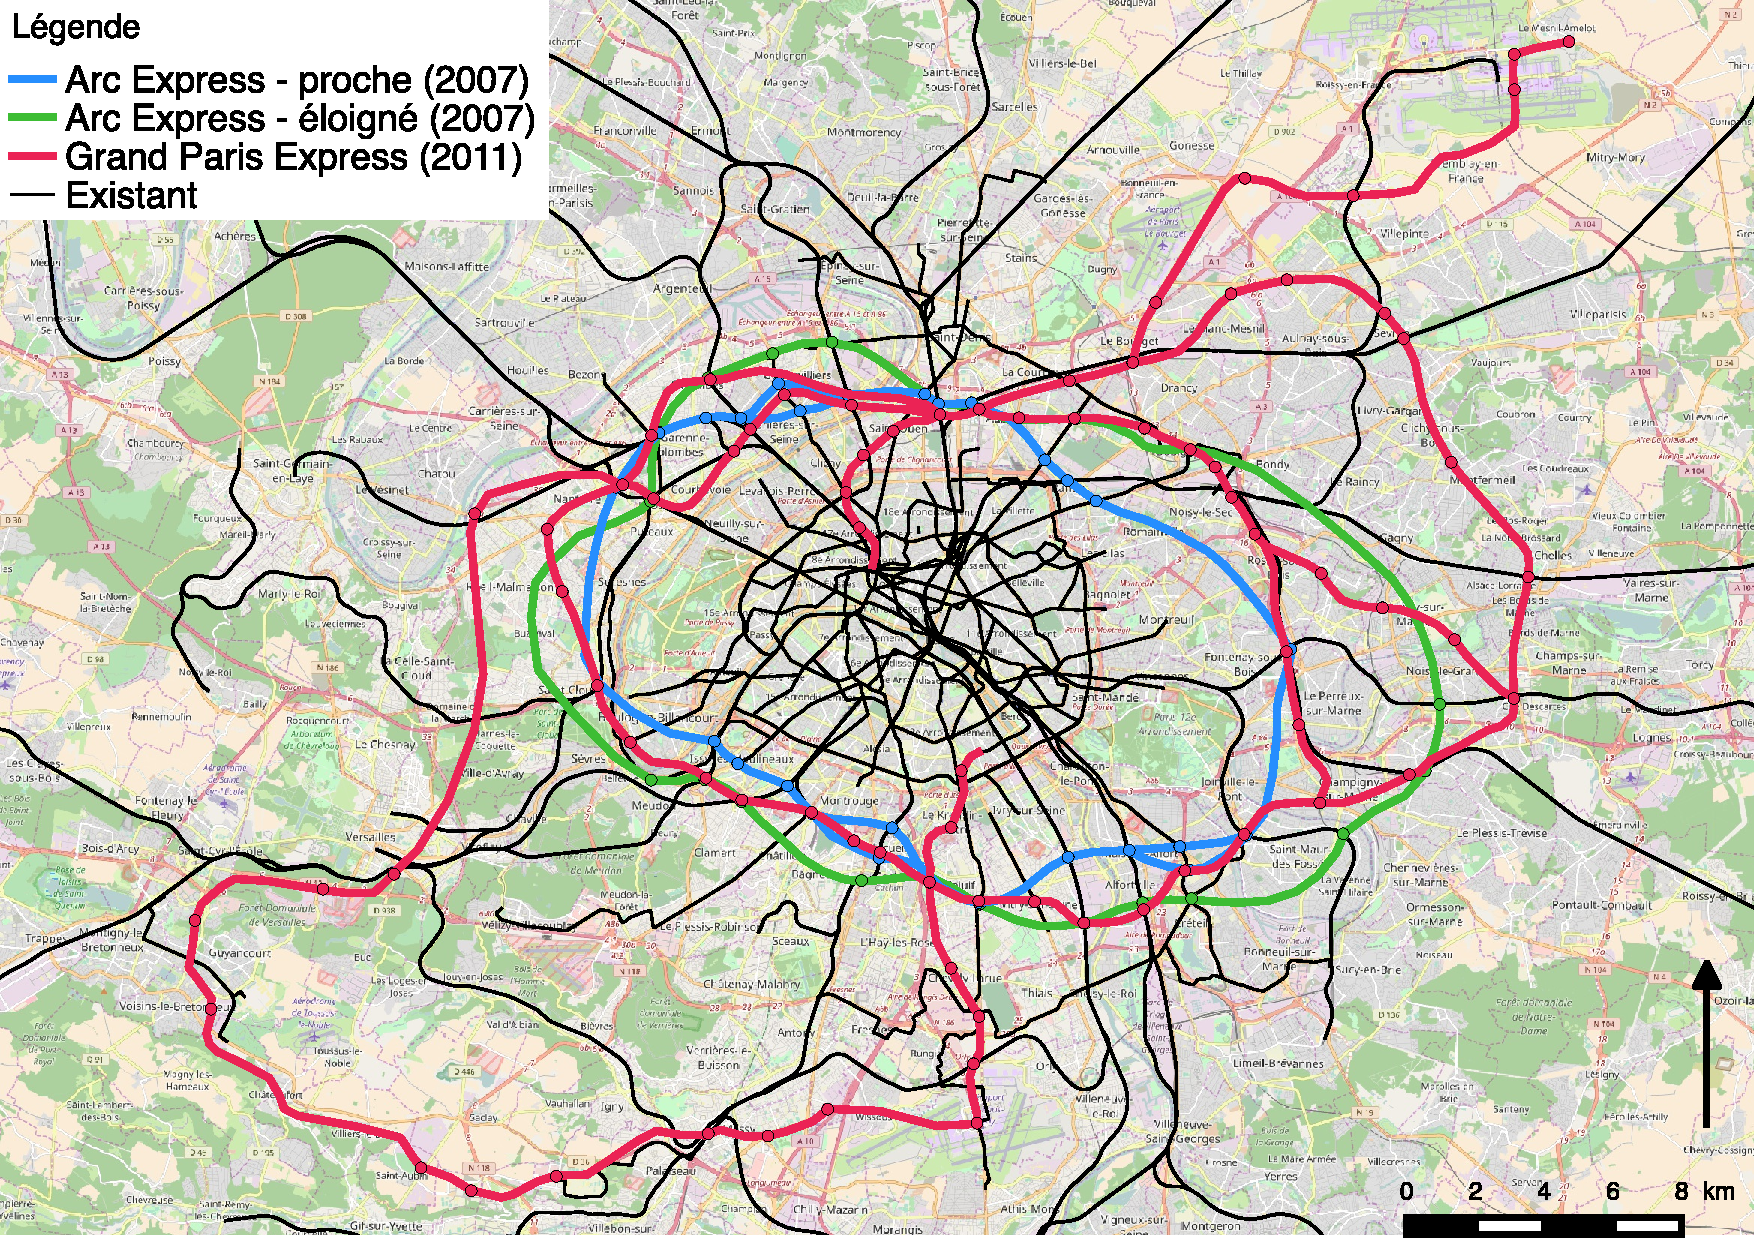
\includegraphics[width=12cm]{Figures/GrandParisRealEstate/reseaux}
\caption[][Projets de transport successifs du Grand Paris]{}{\textbf{Projets de transport successifs de la métropole du Grand Paris.} Nous montrons les deux alternatives du projet Arc Express porté par la région, et le Grand Paris Express (GPE) porté par l'état. Le Réseau du Grand Paris, précurseur du GPE, n'est pas montré ici pour des raisons de visibilité à cause de sa proximité avec celui-ci.}
\label{fig:projects}
\end{figure*}
%%%%%%%%%%%%%%%



\subsubsection{Results}{Résultats}


% note : étude de l'accessibilité pondérée : pas conclusif au regard des réseaux de transports car pas sensible à un changement de réseau, majoritairement influencé par les variables territoriales.

% low decay increase absolute correlation (expected ?)





Nous calculons pour chaque projet, le différentiel $\Delta T_i$ d'accessibilité en temps moyen de trajet à partir de chaque IRIS en comparaison à celui dans le réseau sans le projet, défini par $T_i = \sum_k \exp{-t_{ik}/t_0}$ avec $k$ communes, $t_{ik}$ temps de trajet, et $t_0$ paramètre d'atténuation. A chaque projet est associée une date\footnote{2006 pour Arc Express, 2008 pour le Réseau du Grand Paris, 2010 pour le Grand Paris Express}, correspondant environ à l'année d'annonce mature du projet, restant toutefois arbitraire car difficile d'une part à déterminer précisément, un projet n'émergeant pas d'un coup du jour au lendemain, et d'autre part pouvant correspondre à des réalités différentes d'apprentissage du projet par les différents agents économiques (nous faisons donc l'hypothèse réductrice mais nécessaire d'une diffusion sur la majorité des agents dans un temps inférieur à l'année). Nous étudions les corrélations décalées de cette variable avec les variations $\Delta Y_{ij}$ des variables socio-économiques suivantes : population, revenu médian, indice de Gini des revenus, prix moyen des transactions immobilières et montant moyen des crédits immobiliers. Un test de Fisher est effectué pour chaque estimation, et la valeur est fixée nulle si celui-ci n'est pas significatif ($p<0.05$ de manière classique). L'étude avec accessibilité généralisées au sens de Hansen a également été menée mais moins intéressante car très peu sensible à la composante mobilité (réseau et atténuation) par rapport aux variables elle-même, informe uniquement sur des relations entre celles-ci et n'est donc pas présentée ici. Nous présentons en Fig.~\ref{fig:empiricalres} les résultats pour l'ensemble des réseaux et variables. Il est remarquable tout d'abord de noter l'existence d'effets significatifs pour l'ensemble des variables. Des valeurs plus basses du paramètre $t_0$ donnent des corrélations plus fortes en valeur absolue, révélant une possible plus grande importance de l'accessibilité locale sur les dynamiques territoriales. Le comportement de la population montre un pic très détaché correspondant à 2008, laissant supposer un impact du plus vieux projet d'Arc Express sur la croissance de la population, l'effet des autres projets serait alors fallacieux de par leur proximité dans les grands tronçons : cela impliquerait que les zones où ils diffèrent fondamentalement comme le Plateau de Saclay ne soient que très peu sensibles au projet de transport, ce qui confirmerait l'aspect artificiel planifié du développement de ce territoire. Concernant les revenus, on observe un comportement similaire mais négatif, ce qui impliquerait un appauvrissement lié à l'augmentation de l'accessibilité, mais qui semble toutefois s'accompagner d'une baisse des inégalités. Enfin, comme attendu les prix immobiliers sont tirés par l'arrivée potentielle des nouveaux réseaux, effet qui disparait à deux ans pour le Grand Paris Express, suggérant une bulle immobilière passagère. Nous démontrons ainsi l'existence de liens de correlations retardées complexes qu'on nomme causalités en ce sens, entre dynamiques territoriales et dynamiques anticipées des réseaux. Une compréhension plus fine des processus à l'oeuvre est au delà de la portée de cet article, car supposerait des études de terrain qualitatives, des études de cas ciblées, etc. Cet exemple illustre cependant le caractère opérationnel de notre méthode sur un cas d'étude réel.
 

% \cite{guerois2009dynamique} : bulles immobilières locales ?


%%%%%%%%%%%%%%%
\begin{figure*}[h]
%\centering
\hspace{-1cm}
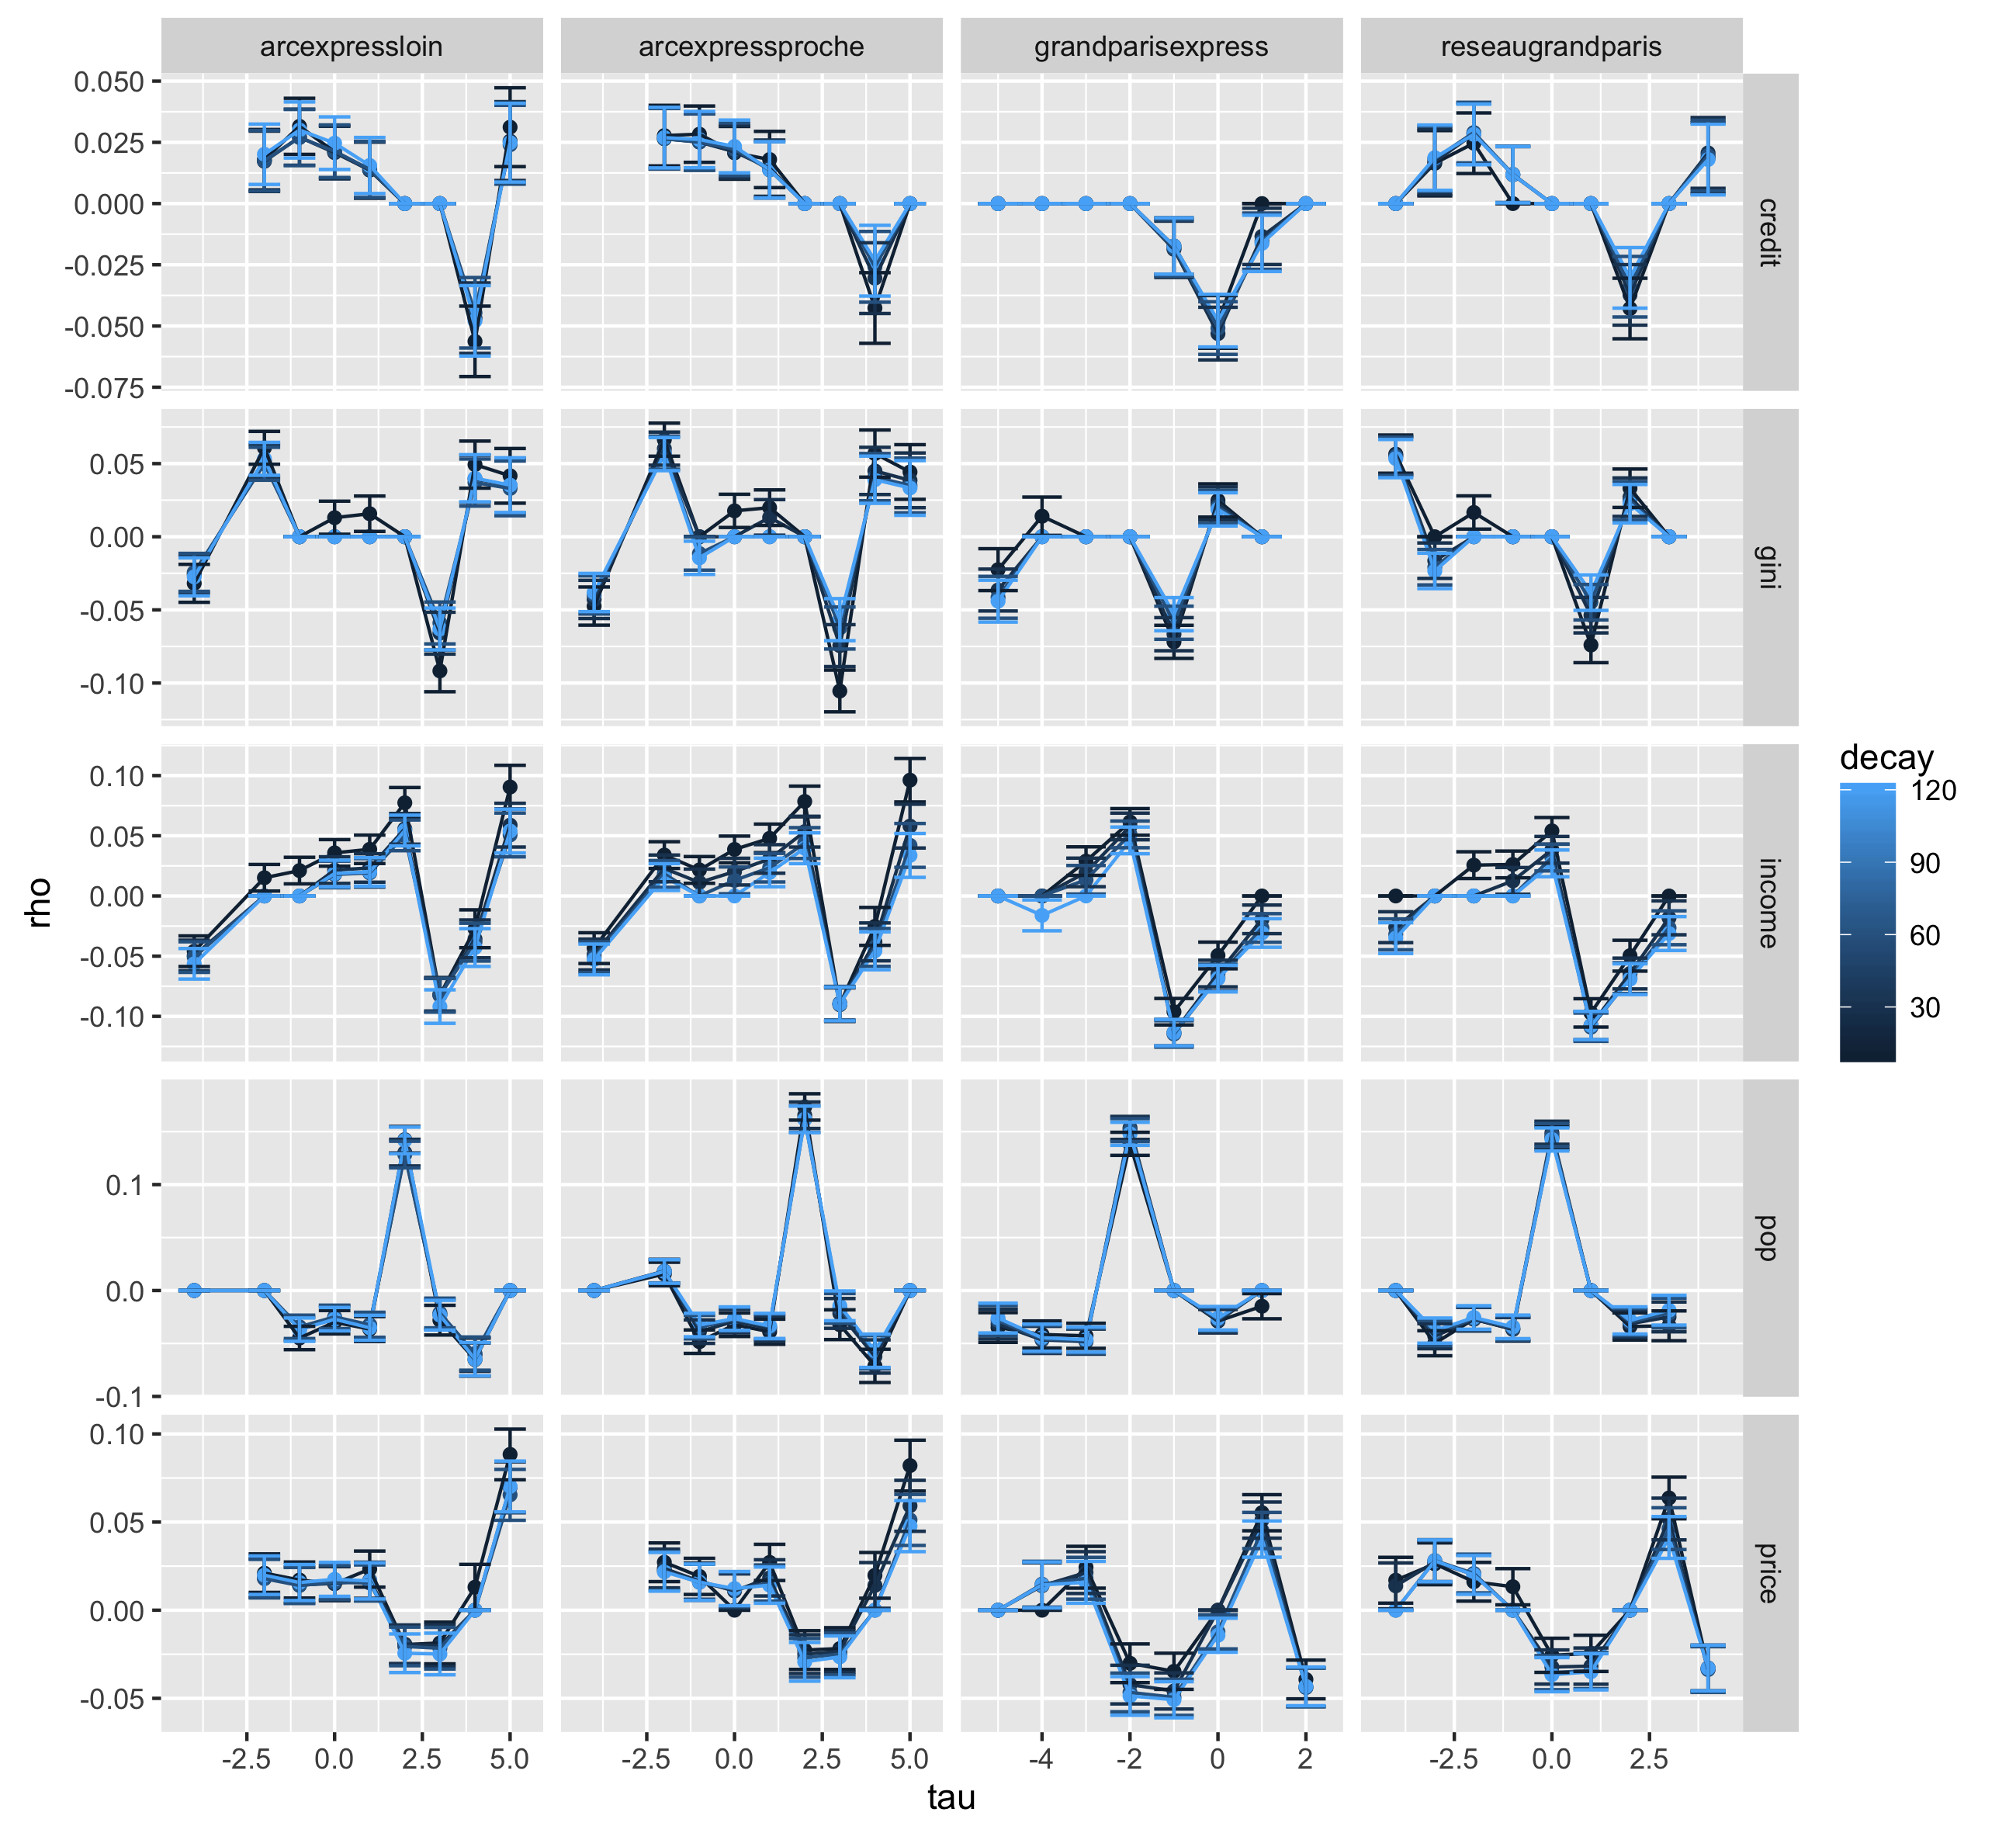
\includegraphics[width=14cm]{Figures/GrandParisRealEstate/laggedcorrs_times_allvars}
\caption[][Corrélations retardées empiriques]{}{\textbf{Corrélations retardées empiriques.} Les graphiques donnent la valeur de la correlation entre le différentiel d'accessibilité en temps de trajet moyen $\Delta T$ pour chaque projet (en colonnes) et le différentiel des différentes variables socio-economiques et de transactions immobilières (en lignes), pour différentes valeurs du paramètre d'atténuation (\texttt{decay}). Les barres d'erreur donnent l'intervalle de confiance à 95\%.}
\label{fig:empiricalres}
\end{figure*}
%%%%%%%%%%%%%%%






%%%%%%%%%%%%%%%
\subsection{Discussion}{Discussion}
%%%%%%%%%%%%%%%


%%%%%%%%%%%%%%%
\subsubsection{Spatio-temporal diffusion}{Diffusion spatio-temporelle}

% STARMA, ondes, ergodicité etc.

L'application de notre approche doit être menée précautionneusement concernant le choix des  échelles, processus et objets d'étude. Typiquement, elle ne sera pas du tout adaptée à la quantification de processus spatio-temporels dont l'échelle temporelle de diffusion est de l'ordre de celle de la fenêtre d'estimation : l'hypothèse de stationnarité est basique. On peut proposer de procéder à des estimations par fenêtres glissantes, mais il faudrait ensuite élaborer une technique de correspondance spatiale pour traquer la propagation des phénomènes. Un exemple d'application concrète à l'impact thématique fort serait une caractérisation d'une composante fondamentale de la Théorie Evolutive des Villes, la diffusion hiérarchique de l'innovation entre les villes~\cite{pumain2010theorie}, en analysant les potentielles dynamiques spatio-temporelles des classifications de brevets comme celle introduite par~\cite{10.1371/journal.pone.0176310}. Il faut noter toutefois qu'il s'agit de questions méthodologiques relativement ouvertes, dont une des manifestations est le lien potentiel entre le caractère non-ergodique des systèmes urbains~\cite{pumain2012urban} et une caractérisation ondulatoire de ces processus.




%%%%%%%%%%%%%%%
\subsubsection{Geographically Weighted Regression}{Regression Géographique Pondérée}

% lien avec GWR ?

Une autre direction de développement et d'applications potentiels se révèle en se tournant vers l'échelle plus locale, et d'explorer une hybridation avec les techniques de Regression Géographique Pondérée~\cite{brunsdon1998geographically}. La détermination par validation croisée ou Critère d'Akaike d'une portée spatiale optimale pour la performance de ce type de modèles pourrait être adaptée dans notre cas pour déterminer une échelle locale optimale sur laquelle les correlations retardées sont les plus significatives, ce qui permettrait de s'extraire du problème de la non-stationnarité prioritairement par l'aspect spatial.


\stars



%%%%%%%%%%%%%%%
%\subsection{Conclusion}{Conclusion}
%%%%%%%%%%%%%%%

%Nous avons proposé une méthode générique de causalité de Granger sur des données territoriales, puis démontré sa potentialité et son caractère opérationnel sur données synthétiques et un cas réel. Nous postulons que l'appareillage méthodologique simple est un atout pour une certaine généralité, mais que l'application à ces cas complexes présentant des causalités circulaires a un fort potentiel de contribution à la compréhension des dynamiques de ce type de systèmes co-évolutifs.









